\documentclass[zihao=-4]{ctexart}
\usepackage[normalem]{ulem}
\useunder{\uline}{\ul}{}
%********************导言区宏包引入********************
\usepackage{xeCJK}
\usepackage{amssymb}
\usepackage{amsmath}
\usepackage{listings} %代码
\usepackage{graphicx}
\usepackage{multicol} %回车换段
\usepackage{xcolor}
\usepackage{geometry} %页面设置
\usepackage{fontspec}
\usepackage{setspace}
\usepackage{times}
\usepackage{fancyhdr} %页眉页脚
\pagestyle{fancy}
\usepackage{float} %表格位置
\usepackage{titlesec} %设置
\usepackage{titletoc}
\usepackage{ctex}
\usepackage{gbt7714}    %控制参考文献格式为国标
\usepackage{multirow}
\usepackage{booktabs}   %表格相关
\usepackage{setspace}   %设置行距
\usepackage{caption} %caption
\usepackage{subcaption} %子图的caption
\usepackage{changepage} %左右缩进
\usepackage{xurl}
\def\UrlBreaks{%
    \do\/%
    \do\a\do\b\do\c\do\d\do\e\do\f\do\g\do\h\do\i\do\j\do\k\do\l%
    \do\m\do\n\do\o\do\p\do\q\do\r\do\s\do\t\do\u\do\v\do\w\do\x\do\y\do\z%
    \do\A\do\B\do\C\do\D\do\E\do\F\do\G\do\H\do\I\do\J\do\K\do\L%
    \do\M\do\N\do\O\do\P\do\Q\do\R\do\S\do\T\do\U\do\V\do\W\do\X\do\Y\do\Z%
    \do0\do1\do2\do3\do4\do5\do6\do7\do8\do9\do=\do/\do.\do:%
    \do\*\do\-\do\~\do\'\do\"\do\-}
\urlstyle{same}


% for 代码
\definecolor{mygreen}{rgb}{0,0.6,0}
\definecolor{mygray}{rgb}{0.5,0.5,0.5}
\definecolor{mymauve}{rgb}{0.58,0,0.82}


\graphicspath{ {include_picture/}{plots/} }
\let\algorithm\relax
\let\endalgorithm\relax
\usepackage[ruled,vlined]{algorithm2e}%[ruled,vlined]{
\usepackage{algpseudocode}
\renewcommand{\algorithmicrequire}{\textbf{Input:}} 
\renewcommand{\algorithmicensure}{\textbf{Output:}}
%\renewcommand\thepage{\zihao{-5} ~\arabic{page}~}%页码字号

%定义两个arg
\DeclareMathOperator*{\argmax}{arg\,max}
\DeclareMathOperator*{\argmin}{arg\,min}
\DeclareCaptionLabelSeparator{mysep}{\space\space}  %自定义caption格式
\captionsetup[figure]{font={small}, labelfont=bf, labelsep=mysep, textfont=bf}   %图片caption格式
\captionsetup[table]{font={small}, labelfont=bf, labelsep=mysep, textfont={bf}}   %表格caption格式
\bibliographystyle{gbt7714-numerical} %修改了title斜体内容

\usepackage[colorlinks,bookmarksopen,bookmarksnumbered,citecolor=blue, urlcolor=blue]{hyperref}
\hypersetup{
    linkcolor=black
}

%********************导言区宏包引入********************
%********************第三方字体引入********************
%\setCJKmainfont[Path=fonts/,BoldFont=simhei.ttf,ItalicFont=simkai.ttf,SlantedFont=simfang.ttf]{simsun.ttc}
%中文字体涵盖黑体、宋体、楷体、仿宋
\setmainfont[Path=fonts/, 
BoldFont = times-new-roman-bold.ttf,
ItalicFont = times-new-roman-italic.ttf,
BoldItalicFont = times-new-roman-bold-italic.ttf
]{times-new-roman.ttf}
\setmonofont[Path=fonts/]{Courier New.ttf}
\setCJKfamilyfont{hwzs}[Path=fonts/]{STKzhongsong.ttf}%使用STZhogsong华文中宋字体
\newcommand{\zhongsong}{\CJKfamily{hwzs}}
\setCJKfamilyfont{hwxw}[Path=fonts/]{STKxinwei.ttf} % XSP 2023/3/3:
\newcommand{\xinwei}{\CJKfamily{hwxw}}              %  使用STZxinwei华文新魏字体.

%********************第三方字体引入********************


%********************中文字号设置********************
%\newcommand{\chuhao}{\fontsize{42pt}{\baselineskip}\selectfont}
\newcommand{\chuhao}{\fontsize{42pt}{0}}
\newcommand{\xiaochu}{\fontsize{36pt}{0}}
\newcommand{\yihao}{\fontsize{28pt}{0}}
\newcommand{\erhao}{\fontsize{21pt}{0}}
\newcommand{\xiaoer}{\fontsize{18pt}{0}}
\newcommand{\sanhao}{\fontsize{16pt}{0}}
\newcommand{\sihao}{\fontsize{14pt}{0}}
\newcommand{\xiaosi}{\fontsize{12pt}{0}}
\newcommand{\wuhao}{\fontsize{10.5pt}{0}}
\newcommand{\xiaowu}{\fontsize{9pt}{0}}
\newcommand{\liuhao}{\fontsize{8pt}{0}}
\newcommand{\qihao}{\fontsize{5.25pt}{0}}

% 个人信息 自定义命令 固定长度下划线
\newcommand\ful[2][4cm]{\underline{\makebox[#1][c]{#2}}}
%********************中文字号设置********************


%********************代码段********************
% https://www.cnblogs.com/PiaYie/p/15720770.html
\renewcommand{\lstlistingname}{代码}
\lstset{ %
  backgroundcolor=\color{white},   % choose the background color; you must add \usepackage{color} or \usepackage{xcolor}
  basicstyle=\footnotesize,        % the size of the fonts that are used for the code
  breakatwhitespace=false,         % sets if automatic breaks should only happen at whitespace
  breaklines=true,                 % sets automatic line breaking
  captionpos=bl,                    % sets the caption-position to bottom
  commentstyle=\color{mygreen},    % comment style
  deletekeywords={...},            % if you want to delete keywords from the given language
  escapeinside={\%*}{*)},          % if you want to add LaTeX within your code
  extendedchars=true,              % lets you use non-ASCII characters; for 8-bits encodings only, does not work with UTF-8
  frame=single,                    % adds a frame around the code
  keepspaces=true,                 % keeps spaces in text, useful for keeping indentation of code (possibly needs columns=flexible)
  keywordstyle=\color{blue},       % keyword style
  %language=Python,                 % the language of the code
  morekeywords={*,...},            % if you want to add more keywords to the set
  numbers=left,                    % where to put the line-numbers; possible values are (none, left, right)
  numbersep=5pt,                   % how far the line-numbers are from the code
  numberstyle=\tiny\color{mygray}, % the style that is used for the line-numbers
  rulecolor=\color{black},         % if not set, the frame-color may be changed on line-breaks within not-black text (e.g. comments (green here))
  showspaces=false,                % show spaces everywhere adding particular underscores; it overrides 'showstringspaces'
  showstringspaces=false,          % underline spaces within strings only
  showtabs=false,                  % show tabs within strings adding particular underscores
  stepnumber=1,                    % the step between two line-numbers. If it's 1, each line will be numbered
  stringstyle=\color{orange},     % string literal style
  tabsize=2,                       % sets default tabsize to 2 spaces
  literate={-}{{\textendash}}{1}
  %title="No name code"                   % show the filename of files included with \lstinputlisting; also try caption instead of title
}
%********************代码段********************


%********************页边距设置********************
\geometry{left=3cm,right=2cm,top=2.5cm,bottom=2.5cm}
\geometry{a4paper} % xsp 2023/3/7: 调整纸张大小为A4
%********************页边距设置********************

%********************段间距设置********************
\newcommand{\setParDis}{\setlength {\parskip} {0pt} }
%请在每部分使用这个
%********************段间距设置********************

%********************

\begin{document}
%********************页眉页脚设置********************
\lhead{}%设置左页眉为空
\rhead{}%设置左页眉为空
\setlength{\headwidth}{\textwidth}% 2023/3/3 XSP: 页眉长度适应文本
%********************页眉页脚设置********************


%********************标题格式设置********************

%\setcounter{secnumdepth}{0}%该命令取消了章标题前数字label

\CTEXsetup[name={,、},number={\chinese{section}}]{section}
\CTEXsetup[name={（,）},number={\chinese{subsection}}]{subsection}
\CTEXsetup[name={,.},number={\arabic{subsubsection}}]{subsubsection}% 不加会导致目录格式错误
% 设置subsubsection等格式
% \titleformat{\section}[block]{\sanhao\bfseries\centering}{\chinese{section}、}{0pt}{}[]
% \titleformat{\subsection}[block]{\sihao\bfseries}{（\chinese{subsection}）}{0pt}{}[]
% \titleformat{\subsubsection}[block]{\xiaosi\bfseries}{\arabic{subsubsection}、}{0pt}{}[]
\titleformat{\section}[block]{\sanhao\heiti\centering}{\chinese{section}、}{0pt}{}[]    % XSP 2023/3/3:
\titleformat{\subsection}[block]{\sihao\heiti}{（\chinese{subsection}）}{0pt}{}[]       %   将正文标题字体由加粗
\titleformat{\subsubsection}[block]{\xiaosi\heiti}{\arabic{subsubsection}.}{0pt}{}[]   % 修改为黑体。
\titlespacing{\section}{0pt}{25pt}{12pt}
\titlespacing{\subsection}{0pt}{7pt}{7pt}
\titlespacing{\subsubsection}{0pt}{5pt}{4pt}

\titlecontents{section}[1.6em]{\addvspace{2pt}\filright}
{\contentspush{\thecontentslabel\hspace{0.8em}}}
{}{\titlerule*[8pt]{.}\contentspage}

\titlecontents{subsection}[3.2em]{\addvspace{2pt}\filright}
{\contentspush{\thecontentslabel\hspace{0.8em}}}
{}{\titlerule*[8pt]{.}\contentspage}

\titlecontents{subsubsection}[6.4em]{\addvspace{2pt}\filright}
{\contentspush{\thecontentslabel\hspace{0.8em}}}
{}{\titlerule*[8pt]{.}\contentspage}
%********************标题格式设置********************

%\setcounter{section}{-3}  %标题计数器
%\stepcounter{section}

%*******************行间距段前段后*******************
\linespread{1.8}
%行间距为实际行间距乘以1.2,如此处实际为1.5倍行距
\setlength{\parskip}{0.5\baselineskip}
%*******************行间距段前段后*******************



%********************封面部分********************
%
%     论文题目：应准确、鲜明、简洁，能概括整个论文中最主要和最重要的内容。
% 题目不超过20个中文字，若语意未尽，可用副标题补充说明。副标题应处于从属
% 地位，一般可在题目的下一行用破折号“——”引出。论文题目应避免使用不常用缩
% 略词、首字母缩写字、字符、代号和公式等。
%
% \def\Fengru{第三十四届“冯如杯”竞赛主赛道}
\def\CourseName{《并行程序设计A》}
\leftline{\includegraphics[scale=1]{include_picture/xiaohui.png}} % XSP 2023/3/3: 取消校徽段首缩进
%格式控制部分
% \par \  
% \par \
% \par \
\vspace{32pt}
\begin{center}
\includegraphics[height=2.25cm, width=12.78cm, scale=1]{include_picture/xiaoming.png}
\end{center}
%格式控制部分
\vspace{12pt}

\begin{spacing}{3}
    % \erhao
    \begin{center}
      {
        \fontsize{22pt}{3}\selectfont
        \zhongsong{MPI编程实验报告} %黑体这样调用，其余字体同理
      } 
        % \zhongsong{“冯如杯”竞赛主赛道项目是什么}
    \end{center}
    \rightline{\xinwei\sanhao{\CourseName 课程报告}} % XSP 2023/3/3: 副标题二号华文新魏居右

    \vspace{2cm}
    \begin{center}
    \textbf{\sanhao
        \makebox[2cm][s]{学院}：\ful[5cm]{软件学院}\\
        \makebox[2cm][s]{班级}：\ful[5cm]{ZY25211}\\
        \makebox[2cm][s]{姓名}：\ful[5cm]{刘益洲}\\
        \makebox[2cm][s]{学号}：\ful[5cm]{ZY2521110}\\
    }
    \end{center}

\end{spacing}
%格式控制部分
% \par \ 
% \par \
% \par \ 
% \par \
% \par \ 
% \par \
% \begin{center}
%     \sihao
%     \textbf{学院：计算机学院}
%     \par \ 
%     \textbf{本模板原作者：Someday}
% \end{center}

%格式控制部分
\par \ 
\begin{center}
\sanhao
\centerline{\heiti{}}%封面年月去掉
\end{center}

\pagenumbering{gobble} %封面无页码
%\thispagestyle{empty}


\renewcommand{\headrulewidth}{0pt}%没有页眉装饰线
\clearpage
\pagenumbering{roman} %摘要目录页小写罗马
 

%********************目录部分********************
\clearpage
\tableofcontents
\clearpage
%********************目录部分********************



\renewcommand{\headrulewidth}{0.4pt} %恢复页眉装饰线

%********************正文页眉部分********************
%\lhead{} 
\chead{\xiaowu \CourseName 课程报告} %设置居中页眉
%********************正文页眉部分********************

\pagenumbering{arabic} %正文页码从1开始，用阿拉伯数字
\setcounter{page}{1} 

\section{实验环境}
\setParDis %设置段间距为 0
\begin{spacing}{1.5}

本实验在表~\ref{tab:exp-env}、表~\ref{tab:exp-sw}所列环境下完成；表中数值由集群配置说明及容器内 \texttt{lscpu}、\texttt{nproc}、\texttt{uname} 等命令整理得到。

\begin{table}[H]
\small
\centering
\caption{实验硬件与系统环境}
\label{tab:exp-env}
\begin{tabular}{ll}
\toprule
名称 & 版本或配置 \\
\midrule
集群 & Kubernetes \\
工作负载 & Pod \\
containerd & 2.2.1 \\
Kubelet & v1.35.2 \\
\midrule
Pod CPU 配额 & 70 核 \\
Pod 内存配额 & 64\,GiB \\
CPU 绑核 & 未开启 \\
\midrule
处理器 & Intel Xeon Gold 6148 @ 2.40\,GHz（2 路，20 核/路，HT） \\
逻辑 CPU & 80 \\
架构 & x86\_64 \\
\midrule
Ubuntu & 24.04.1 LTS \\
Linux 内核 & 5.15.0-170-generic \\
Locale & \texttt{C.UTF-8} \\
\bottomrule
\end{tabular}
\end{table}

MPI 程序所用编译与运行环境见表~\ref{tab:exp-sw}（仅 MPI，不使用 OpenMP）。

\begin{table}[H]
\small
\centering
\caption{MPI 与编译工具环境}
\label{tab:exp-sw}
\begin{tabular}{ll}
\toprule
名称 & 版本或配置 \\
\midrule
GCC & 13.3.0 \\
G++ & 13.3.0 \\
Open MPI & 4.1.6 \\
mpicc / mpicxx & Open MPI 4.1.6（GCC 13.3.0） \\
mpirun & 4.1.6 \\
mpirun 启动选项 & \texttt{--use-hwthread-cpus} \\
GNU Make & 4.3 \\
glibc & 2.39 \\
编译优化 & \texttt{-O3} \\
\bottomrule
\end{tabular}
\end{table}

\section{实验内容与方法}

\subsection{实验内容}
第 3 次作业要求使用 MPI 实现矩阵并行乘法，编程语言为 C/C++。方阵规模 \(N\times N\) 满足 \(N\ge 8000\)，矩阵元素为双精度浮点数；按三矩阵各占用约 \(N^2\) 个双精度元素估算，\(N=8000\) 时单矩阵约 512\,MiB，三矩阵合计约 1.5\,GiB 量级（作业说明中给出的约 480\,MB 为常用估算口径）。实验需完成并行程序，并与串行实现对比，给出加速比；统计计算时间时应排除矩阵初始化、文件 I/O 等数据准备时间。此外需考察并行程序的可扩展性，例如改变 MPI 进程数、关注数据划分带来的局部性等因素。

\subsection{实验方法}

\paragraph{并行模型与算法}
MPI 用于在单节点、多进程下组织并行（\texttt{mpirun -np $p$}，Open MPI 4.1.6）。将 \(N\times N\) 矩阵 \(A,B,C\) 在行列方向各划分为 \(P_r\times P_c\) 个子块（\(P_r P_c=p\)，\(p\) 分解为近似方阵的进程网格），记块下标为 \(i,j,k\)，子块 \(A_{i,k}\)、\(B_{k,j}\)、\(C_{i,j}\) 的规模随 \(N\) 与余数分配略有差别，但满足块矩阵乘法（与作业示意图一致）：
\begin{equation*}
C_{i,j}=\sum_{k=0}^{P_c-1} A_{i,k} B_{k,j}.
\end{equation*}
进程按二维坐标 \((i,j)\) 编号，\(\mathrm{rank}=i\cdot P_c+j\)，负责累加本地 \(C_{i,j}\)。对每个 \(k\)，自进程 \((i,k)\) 接收 \(A_{i,k}\)、自 \((k,j)\) 接收 \(B_{k,j}\)（若即为拥有者则直接访问），完成子块乘加后写入 \(C_{i,j}\)。乘加结束后，各进程将 \(C_{i,j}\) 发往根进程，在 rank 0 上拼装为完整的 \(N\times N\) 矩阵 \(C\)，从而构成完整的并行矩阵乘法流程。\(p=1\) 时无进程间通信。本地子块内部仍用朴素三重循环，不在子块内再做 cache 分块。

\paragraph{进程间通信}
本实验通信分为三阶段（见表~\ref{tab:mpi-comm}），均计入一次完整并行矩阵乘法的耗时 \(T_p\)：子块分发、按 \(k\) 轮的块乘加通信、结果汇聚。仅根进程上 \(A,B\) 的伪随机初始化在 \texttt{MPI\_Wtime} 之前完成，以符合作业“排除数据准备”的要求。

\begin{table}[H]
\small
\centering
\caption{MPI 矩阵乘法的进程间通信阶段}
\label{tab:mpi-comm}
\begin{tabular}{llp{5.8cm}}
\toprule
阶段 & 是否计入 \(T_p\) & 内容与原语 \\
\midrule
数据初始化 & 否 & 根进程生成 \(A,B\) 元素值（在 \texttt{MPI\_Wtime} 之前） \\
子块分发 & 是 & \(A_{i,k}\) 发往 \((i,k)\)，\(B_{k,j}\) 发往 \((k,j)\)（\texttt{MPI\_Send}/\texttt{MPI\_Recv}） \\
块乘加通信 & 是 & 对每个 \(k\)：交换 \(A_{i,k}\)、\(B_{k,j}\) 并本地累加 \(C_{i,j}\) \\
结果汇聚 & 是 & 各进程将 \(C_{i,j}\) 发往 rank 0，拼装为全局 \(C\) \\
\bottomrule
\end{tabular}
\end{table}

\paragraph{实验设计}
在 Pod 配额（70 CPU、64\,GiB 内存、未绑核）内考察进程数可扩展性，其余因素固定，如表~\ref{tab:exp-design}。

\begin{table}[H]
\small
\centering
\caption{矩阵乘法实验因素设计}
\label{tab:exp-design}
\begin{tabular}{ll}
\toprule
名称 & 取值或说明 \\
\midrule
矩阵阶数 \(N\) & 8000（满足 \(N\ge 8000\)，三矩阵约 1.5\,GiB） \\
进程数 \(p\) & 64, 32, 16, 8, 4, 2, 1（从大到小依次测试） \\
进程网格 & \(P_r\times P_c=p\)，\(P_r\ge P_c\)，因子分解尽量接近方阵 \\
mpirun 选项 & \texttt{--use-hwthread-cpus}（见下文） \\
并行策略 & 二维块划分，\(C_{i,j}=\sum_k A_{i,k}B_{k,j}\) \\
数据类型 & \texttt{double}，行主序存储 \\
数据生成 & 根进程确定性初始化（\texttt{MPI\_Wtime} 之前） \\
计时区间 & 子块分发 + 各 \(k\) 子块收发与乘加 + \(C\) 汇聚 \\
排除项 & 矩阵元素初始化、文件 I/O 与写盘 \\
重复次数 & 每个 \((N,p)\) 配置 5 次，取 \texttt{time\_sec} 算术平均 \\
编译选项 & \texttt{mpicc -O3 -std=c11} \\
\bottomrule
\end{tabular}
\end{table}

进程数取 2 的幂直至 64（如 \(p=8\) 对应 \(2\times4\) 网格），\(p=1\) 作为 \(T_1\)。Pod 申请 70 CPU 是为减少同节点其它任务干扰，实验进程数最大仍为 64。各进程常驻内存约为一个 \(C_{i,j}\) 子块，乘加阶段另需缓冲区存放当前 \(A_{i,k}\)、\(B_{k,j}\)，总占用随 \(p\) 增大而分散。

\paragraph{Open MPI 的 slot 限制及处理}
实验初期直接执行 \texttt{mpirun -np 64 ./matmul\_mpi 8000} 时，Open MPI 报错：\emph{not enough slots available}。Open MPI 用 slot 估计本机可启动的进程数；默认常按物理核数记账（本机约 40），低于容器内可见的逻辑 CPU 数（80）。从硬件上讲，一个逻辑 CPU 通常可运行一个 MPI 进程；因此本实验在 \texttt{mpirun} 中增加 \texttt{--use-hwthread-cpus}，按逻辑 CPU 数分配 slot，使 \(p\le 64\) 的测试可以正常启动。基准脚本与手工运行均采用该选项（见表~\ref{tab:exp-design}、表~\ref{tab:exp-sw}）。

\paragraph{评价指标与流程}
记第 \(p\) 个配置的平均耗时为 \(T_p\)，加速比 \(S_p=T_1/T_p\)，并行效率 \(E_p=S_p/p\)。流程：（1）\texttt{make} 生成 \texttt{matmul\_mpi}；（2）每次执行 \texttt{./bench\_matmul\_mpi.sh <rep>} 仅跑一轮，按 \(p=64,32,\ldots,1\) 依次测试；\texttt{mpirun} 带 \texttt{--use-hwthread-cpus}；结果追加至 \texttt{results/matmul\_bench.csv}；同一轮内相邻两次运行间隔 10\,s；（3）绘图并分析 \(S_p\)、\(E_p\)。分析时结合子块通信次数（每个 \((i,j)\) 需 \(P_c\) 轮 \(A/B\) 子块数据）、负载均衡与局部性进行讨论。

\section{实验过程}

\subsection{MPI 块矩阵乘法实现要点}
程序将 \(p\) 分解为 \(P_r\times P_c\)，建立逻辑坐标 \texttt{(proc\_row, proc\_col)}。根进程在计时外初始化 \(A,B\) 后，\texttt{MPI\_Wtime} 计时区间内依次完成：把 \(A_{i,k}\)、\(B_{k,j}\) 分发到各拥有进程；对每个 \(k\in[0,P_c)\) 交换子块并累加 \(C_{i,j}\)；将各 \(C_{i,j}\) 汇聚为 rank 0 上的完整 \(C\)。子块乘法核心如代码~\ref{lst:block-gemm} 所示。

\begin{lstlisting}[language=C,caption={子块乘加（节选）},label={lst:block-gemm}]
for (int ii = 0; ii < rows_a; ii++)
  for (int jj = 0; jj < cols_b; jj++) {
    double sum = C_local[ii * cols_b + jj];
    for (int kk = 0; kk < cols_a; kk++)
      sum += A_sub[ii * cols_a + kk] * B_sub[kk * cols_b + jj];
    C_local[ii * cols_b + jj] = sum;
  }
\end{lstlisting}

对每个 \(k\)，拥有 \(A_{i,k}\) 的进程 \((i,k)\) 向同行其余进程 \texttt{MPI\_Send} 子块；\((i,j)\)（\(j\neq k\)）\texttt{MPI\_Recv} 接收。\(B_{k,j}\) 由 \((k,j)\) 向同列其余进程发送、\((i,j)\)（\(i\neq k\)）接收。

计时区间内，函数 \texttt{gather\_C\_blocks} 将本地 \(C_{i,j}\) 发往 rank 0，拼装为完整 \(C\)，作为一次矩阵乘法的收尾步骤。

\subsection{计时与重复实验流程}
\texttt{MPI\_Wtime} 在根进程完成 \(A,B\) 初始化之后启动，在 \(C\) 汇聚结束之后停止；输出的 \texttt{time\_sec} 覆盖分发、乘加相关通信与汇聚，不含元素初始化。批量实验由脚本对各 \(p\) 调用 \texttt{mpirun}；重复实验通过多次执行 \texttt{bench\_matmul\_mpi.sh <rep>} 完成，解析 \texttt{time\_sec} 取平均。

\subsection{程序编译与运行}
使用 \texttt{mpicc} 编译，例如 \texttt{mpicc -O3 -std=c11 -o matmul\_mpi matmul\_mpi.c}。运行示例：
\texttt{mpirun --use-hwthread-cpus -np 64 ./matmul\_mpi 8000}。
可执行文件与脚本置于 \texttt{h3/} 目录，测数写入 \texttt{h3/results/}。

\section{实验结果与分析}

本节将在完成实测后填入不同 MPI 进程数下的 \(T_p\)、\(S_p\) 与 \(E_p\)，并结合表~\ref{tab:matmul-bench} 与耗时/加速比曲线分析可扩展性。分析时将讨论：随 \(P_c\) 增大子块通信轮次增加的影响、二维划分下的负载均衡，以及子块规模变小时缓存局部性对加速比的作用。

\begin{table}[H]
\small
\centering
\caption{MPI 矩阵乘法性能结果（\(N=8000\)，平均值，单位秒；待填入实测数据）}
\label{tab:matmul-bench}
\begin{tabular}{rrrrr}
\toprule
进程数 \(p\) & 平均耗时 \(T_p\) & 加速比 \(S_p\) & 并行效率 \(E_p\) \\
\midrule
\multicolumn{5}{c}{（实验完成后填写）} \\
\bottomrule
\end{tabular}
\end{table}

% 完成实验后取消注释并放入 plots/ 下图：
% \begin{figure}[H]
%   \centering
%   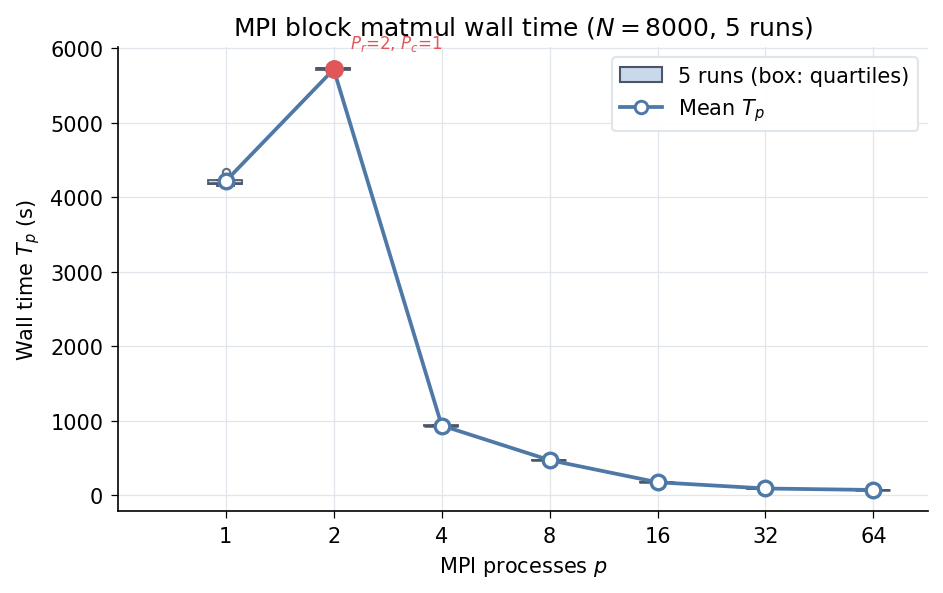
\includegraphics[width=0.85\linewidth]{matmul_time_vs_procs.png}
%   \caption{矩阵乘法耗时与加速比随进程数变化}
%   \label{fig:matmul-curves}
% \end{figure}

\end{spacing}

\end{document}
